\documentclass{article}
\usepackage{fullpage}
\usepackage{graphicx}
\usepackage{titlesec}
\usepackage{hyperref}
\hypersetup{colorlinks=true,linkcolor=blue}
\title{GSAS Refinement Commands}
\setcounter{secnumdepth}{0}
\pagestyle{plain} % No headers, just page numbers

\begin{document}

\begin{center}

\pagenumbering{roman}


\verb=GSAS Refinement Commands=
\end{center}

\tableofcontents

\pagebreak


\pagenumbering{arabic}
\setcounter{page}{1}

\section{About this document}
\begin{center}
AT THIS POINT IN TIME - IF YOU RECEIVE THIS DOCUMENT TREAT IT AS CONFIDENTIAL SINCE THIS IS NOT OFFICIALLY RELEASED - YOU ARE A TEST PERSON HERE! PLEASE DO NOT DISTRIBUTE THE DOCUMENTATION OR THE SCRIPT FILES OUTSIDE YOUR GROUP!  DIRECT INTERESTED PARTIES TO SVEN VOGEL!\\
\end{center}
Send comments to: \href{mailto:sven@lanl.gov}{sven@lanl.gov} \\ \\
\textbf{\large{Why?}} \\ \\
In many cases LANSCE users (or users at other facilities) leave the site with much more than one data set. Data analysis becomes a bottleneck towards publication. Even if one dataset gets analyzed successfully with GSAS, the user might not really remember what he did in the 1258 refinement steps shown in the header of POWPLOT (and knowingly clipped off in presentations by experienced users but innocently left on by new users...). By packaging the analysis into a script we hope that we can help to:
\begin{itemize}
	\item apply the same or very similar analysis to multiple datasets from a parametric study
  \item self-document the refinement strategy (parameter turn-on sequence)
	\item prevent users from having to use the notorious menu tree of EXPEDT
	\item boost the user's ability to analyze data by delivering a template for the analysis from which a user can start

\end{itemize}

\section{Prerequisites}
\begin{itemize}
	\item This package aims at automating GSAS, therefore, a running GSAS is required. To test this, at the command line from which you wish to run this (mouse junkies - this will NOT be your cup of tea� but maybe we can pull you into the great land of command lines) change into a folder with GSAS data and try to plot it in rawplot by typing in rawplot. If this fails with a file not found error, GSAS is either not installed or not in the search path. If it plots, but doesn't have text around the graph, the PGPLOT\_FONT variable is not set. Another missing bit could be the GSAS variable, in which case GSAS wouldn't know where to look for the scattering length etc. All this is documented in the README file coming with GSAS, but who reads those these days...
	\item The 2nd prerequisite is a working understanding of GSAS by the user. If you don't know what GSAS does and how it works, this here will be of little help, it might be even dangerous... We strongly suggest you work at least through the excellent tutorials that come with GSAS to get an idea what GSAS does.

\end{itemize}

\subsection{Linux or Windows?}

We found that the same stuff runs a lot (factor 2 up to 5) faster when a given system runs under Linux. Using the bash shell provides much easier access for fast development of tools like this than the windows shell.

\subsection{Linux/Mac/Unix Installation}

\begin{itemize}
	\item Copy the scripts into an appropriate folder and add it to the path. Done.
ok, maybe not completely. Make sure you have LaTex installed (punch in ``latex'' at a command prompt, it should come up with a LaTeX prompt). If you want to plot the results of a multi-run analysis using gsas\_plot\_overview, make sure you have gnuplot installed.
\end{itemize}

\subsection{Windows Installation}

\begin{itemize}
	\item Copy the scripts into an appropriate folder, e.g. c:$\backslash$gsas\_language 
	\item Since we need a bash shell, install the cygwin package from (www.cygwin.com).  Download the setup executable and store it in the same folder where you will install cygwin (e.g.c:$\backslash$ cygwin). That way it can be used for future additions and updates. Provide your internet options. If you are working at a government lab, choose a cygwin site at another government lab (.gov) since they are connected with a high-speed backbone. Once you see the ``select packages'' screen (see screenshot below), click on the ``View'' button in the top right corner until you see the ``Full'' view. Besides the basic cygwin, select to install also gnuplot.  Make sure to follow the UNIX end-of-line convention, if in doubt (getting weird error messages when running the gsas scripts such as ``unexpected end of file'' or so), run ``dos2unix'' on your script from the command line.
\begin{figure}[h]
	\centering
		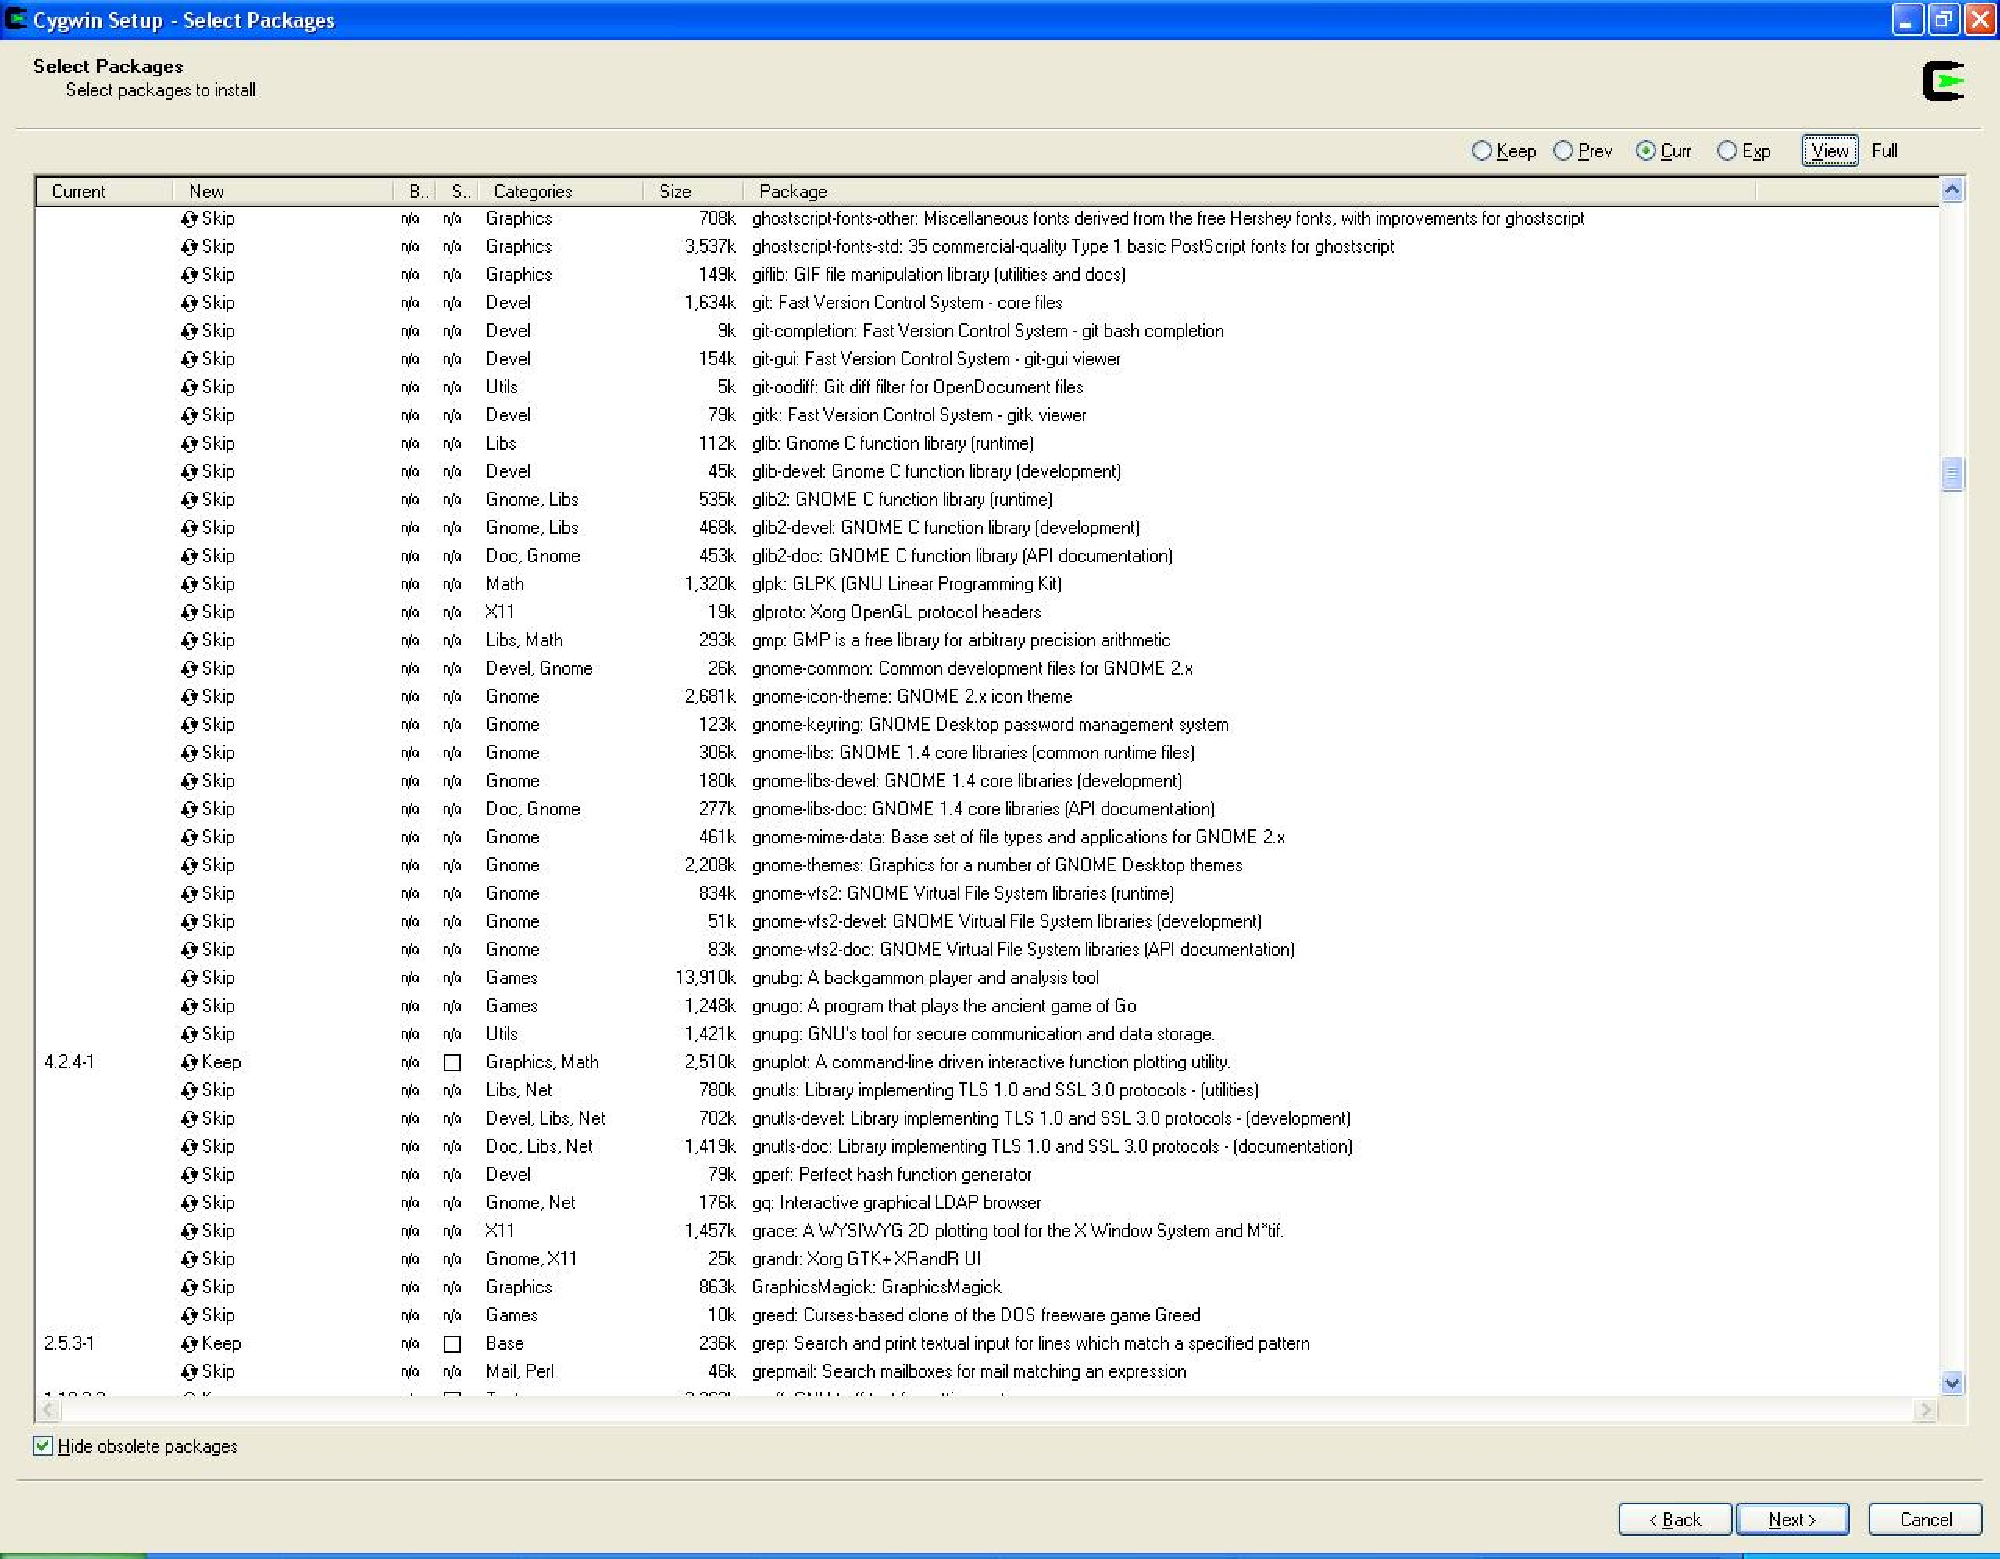
\includegraphics[width=12cm]{Screenshot1.pdf}
	\caption{Selecting packages during Cygwin installation}
	\label{fig:Screenshot1}
\end{figure}

\item Get the GSAS scripts (ZIP files named something like
``gsas\_language.zip'' from Sven -- or steal it from the HIPPO data room computer. Unzip the contents into a folder of your choice.
 Add the folder name to the search path (Control Panel -- System -- Advanced
-- Environment Variables -- PATH)
\item Install LaTex (go to miktex.org to download the basic installation for a Windows system).
\item You may have to install the LaTeX package fullpage manually if your firewall does not allow LaTeX to install it on the fly. If you are using Miktex (Basic MiKtex 2.7), install it into a subfolder of your Miktex installation and refresh the Filename database in the Miktex options.
\end{itemize}

\section{Ready to roll?}

\subsection{Running the demo}
A good start is probably running the demo. This is based on the first tutorial in the GSAS manual; it basically does the same steps described there -- except it takes 20 seconds to run rather than the 2 hours for the average GSAS newbie or 5 minutes for the experienced GSAS user. And it produces a few graphs.\\ \\
Ok, here we go. We assume you installed everything properly. Change to the directory demo, which is a subfolder of the gsas\_language folder. In there, start the script Unix-style with\\ \\
.$\backslash$gsas\_analyze \\ \\
You can look at this file with the editor of your choice (if that choice is wordpad or any other Windows editor and you save the file, make sure to run dos2unix on it before executing it again). 

\subsection{Output Files: Results and Overview}
If really everything is installed nicely (GSAS, gnuplot, latex, ghostscript), you should get four Acrobat PDF files. Three are the results of the three refinements (NICKELxxx.pdf) and one is an overview of the parameters (overview.pdf). The script gsas\_analyze is documented with comments (starting with \# in bash scripts), so not much help needed there. Some more information on the commands is provided in the GSAS Refinement Commands section below. \\ \\
The result PDF files for the refinements show  the data, what was changed, and refinement progress indicators (reduced CHISQ, final variable sum shift) for each refinement step. The data is shown as the usual (non normalized) measured data with fit as well as the plots that are generated if you answer ``yes'' when POWPLOT asks whether you want to see the error analysis. That allows to get a feeling of what the variation of a certain parameter does to the refinement. At the end of the document, you find a list of the refined parameters with errors, which is exactly the PVE file. The PVE file is a good place to collect the parameters of interest for parameter studies etc., which is why it is not deleted at the end of the refinement. The refinement overview files allow you to document a refinement strategy, and they can also tell whether a parameter helps (i.e. the CHISQ goes down substantially) or not. The plot overview in overview.pdf is just meant as an example to show how results of parametric studies can be quickly visualized -- not very meaningful here, but it hopefully gives you an idea how to use it.

\subsection{Problems running refinement script}

\begin{itemize}
	\item If error message ``syntax error...'' or any other strange message occurs on a Windows box, make sure you run ``dos2unix <filename>'' on the script you are running. We recommend using a Unix style editor, either coming with cygwin (install joe for instance, or vi or emacs if you like) or maybe a Windows editor that can handle Unix end-of-line conventions (UltraEdit).
\end{itemize}

\section{Acknowledgements}

Nina Lane provided the majority of this documentation.

\section{GSAS commands}

%gsas_add_atom
\subsection{Add atom}
\begin{quote}
\textit{Function:}\\ 
Inserts an atom\\ \\
\textit{Call with:}\\
\texttt{gsas\_add\_atom <Phase\#> <atom string>} \\ \\
\textit{Inputs:}\\
\begin{tabular}[t]{l l}
\texttt{<Phase\#>} & Phase number\\
\texttt{<atom string>} & Information needed to add an atom: \texttt{<TYPE X Y Z FRAC NAME FLAG U'S>} \\
	& \begin{tabular}[c]{l l}
	\texttt{TYPE} & -- atom type\\
	\texttt{X Y Z} & -- atom fraction on this site\\
	\texttt{FRAC} & -- optional atom name, or / for default\\
	\texttt{FLAG} & -- I for isotropic or A for anisotropic\\
	\texttt{U's} & -- atom temperature factors\\
		& -- either UISO or U11, U22, U33, U12, U13, and U23\\
	\end{tabular}
\end{tabular}
\end{quote}

%gsas_add_histogram
\subsection{Add histogram}
\begin{quote}
\textit{Function:}\\
Inserts a histogram \\ \\
\textit{Call with:}\\
\texttt{gsas\_add\_histogram <filename> <inst prm file> <bank> <min d> <max d>} \\ \\
\textit{Inputs:}\\
\begin{tabular}[t]{l l}
\texttt{<filename>} & Raw histogram input file name\\
\texttt{<inst prm file>} & Instrument parameter file name\\
\texttt{<bank>} & Bank number\\
\texttt{<min d>} & Minimum d-spacing (Angstroms)\\
\texttt{<max d>} & Maximum d-spacing (Angstroms)\\
\end{tabular}
\end{quote}

%gsas_add_phase
\subsection{Add phase}
\begin{quote}
\textit{Function:}\\ 
Inserts a phase \\ \\
\textit{Call with:}\\
\texttt{gsas\_add\_phase <phase name> <space group> <lattice prms>}\\ \\
\textit{Inputs:}\\
\begin{tabular}[t]{l l}
\texttt{<phase name>} & Name of phase\\
\texttt{<space group>} & Space group symbol (ex: P n a 21, P 42/n c m, R -3 c, P 42/m,\\ 
& R -3 m R for rhombohedral setting)\\
\texttt{<lattice prms>} & Real lattice parameters of the new phase (Angstroms)\\
\end{tabular}
\end{quote}

%gsas_change_atom
\subsection{Change atom}
\begin{quote}
\textit{Function:} \\ 
Changes an atom parameter \\ \\ 
\textit{Call with:}\\
\texttt{gsas\_change\_atom <phase\#> <atom range> <parameter name> <value>} \\ \\
\textit{Inputs:} \\
\begin{tabular}[t]{l l}
\texttt{<phase\#>} &  Number of phase for which atom parameters should be changed \\
\texttt{<atom range>} & Atom(s) for which value should be changed: \texttt{<t>}, \texttt{<s>} or \texttt{<s1:s2>} \\
	& \begin{tabular}[c]{l l}
	\texttt{t} & -- for all atoms of type �t�, \\
	\texttt{s} & -- for atom with sequence number �s�,\\ 
	\texttt{s1:s2}& -- for all atoms in sequence number range �s1� to �s2�\\   
	\end{tabular}\\
\texttt{<parameter name>} & Atom parameter which should be changed.  Parameter names allowed:\\
				& \texttt{X Y Z FRAC UISO U11 U22 U33 U12 U13 U23 TYPE NAME}\\
\texttt{<value>} & Value to which parameter should be changed\\ 
\end{tabular}
\end{quote}

%gsas_change background
\subsection{Change background}
\begin{quote}
\textit{Function:} \\
Changes background function \\ \\ 
\textit{Call with:}\\
\texttt{gsas\_change\_background <histogram\#> <bg function> <\# of coeff>}\\ \\
\textit{Inputs:}\\
\begin{tabular}[t]{l l}
\texttt{<histogram\#>} & Number of histogram for which background should be changed\\
\texttt{<bg function>} & Background function to be used  \texttt{<1 �- 9>}\\
	& \begin{tabular}[c]{l l} 
	\texttt{1} & -- Shifted Chebyshev of the first type \\
	\texttt{2} & -- Cosine Fourier series \\
	\texttt{3} & -- Function not defined\\
	\texttt{4} & -- Power series in Q**2n/n!\\
	\texttt{5} & -- Power series in n!/Q**2n\\
	\texttt{6} & -- Power series in Q**2n/n! and n!/Q**2n\\
	\texttt{7} & -- Linear interpolation function\\
 	\texttt{8} & -- Reciprocal interpolation function\\
	\texttt{9} & -- Log interpolation function\\
\end{tabular}\\
\texttt{<\# of coeff>} & Number of background coefficients \texttt{<1 �- 36>} \\
\end{tabular}
\end{quote}

%gsas_change_lattice
\subsection{Change lattice}
\begin{quote}
\textit{Function:} \\
Changes lattice parameter \\ \\
\textit{Call with}\\
\texttt{gsas\_change\_lattice <phase\#> <lattice prms>} \\ \\
\textit{Inputs:} \\
\begin{tabular}[t]{l l} 
\texttt{<phase\#>} &  Number of phase for which lattice parameters should be changed \\
\texttt{<lattice prms>} & Value(s) for new real lattice parameter(s) (Angstroms) \\
\end{tabular}
\end{quote}

%gsas_change_phase_flag
\subsection{Change phase flag}
\begin{quote}
\textit{Function:}\\
Turns phase refinement flag on or off \\ \\
\textit{Call with} \\
\texttt{gsas\_change\_phase\_flag <histogram\#> <phase flag>} \\ \\
\textit{Inputs:}\\
\begin{tabular}[t]{l l}
\texttt{<histogram\#>} & Histogram number for which phase flag should be changed\\
\texttt{<phase flag>} & \texttt{<y>} or \texttt{<n>}, flag whether phase should be in
histogram\\
\end{tabular}
\end{quote}

%gsas_change_phase_scale
\subsection{Change phase scale}
\begin{quote}
\textit{Function:}\\
Changes the phase fraction in all histograms \\ \\
\textit{Call with:}\\
\texttt{gsas\_change\_phase\_scale <phase\#> <value>} \\ \\
\textit{Inputs:} \\
\begin{tabular}[t]{l l}
\texttt{<phase\#>} &  Phase number for which scale should be changed\\
\texttt{<value>} &  New value for phase fraction \\
\end{tabular}
\end{quote}

%gsas_constrain_atom
\subsection{Constrain atom} 
\begin{quote}
\textit{Function:}\\
Constrains atom parameter for specified phase \\ \\
\textit{Call with:}\\
\texttt{gsas\_constrain\_atom <phase\#> <atom prm> <atom\#s>} \\  \\
\textit{Inputs:} \\
\begin{tabular}[t]{l l}
\texttt{<phase\#>} &  Phase number for which atom parameters should be constrained \\
\texttt{<atom prm>} &  Atom parameters which should be constrained (\texttt{FRAC, X, Y, Z, UISO, U11,
MX,} etc.) \\
\texttt{<atom\#s>} &  Atom numbers of the atom set that should be constrained \\
\end{tabular}
\end{quote}

%gsas_constrain_phase
\subsection{Constrain phase}
\begin{quote}
\textit{Function:}\\
Constrains phase to have a constant weight fraction in all histograms \\ \\
\textit{Call with:}\\
\texttt{gsas\_contrain\_phase <phase\#>} \\ \\ 
\textit{Input:}\\
\begin{tabular}[t]{l l}
\texttt{<phase\#>} &  Phase number for which weight fraction should be constrained
\\
\end{tabular}
\end{quote}

%gsas_convert_atom_thermal
\subsection{Convert atom thermal}
\begin{quote}
\textit{Function:} \\
Converts thermal motion parameters of atoms to isotropic or anisotropic \\ \\
\textit{Call with:} \\
\texttt{gsas\_convert\_atom\_thermal <phase\#> <atom range> <flag a/i>} \\ \\   
\textit{Inputs:}\\
\begin{tabular}[t]{l l}
\texttt{<phase\#>} &  Number of phase for which parameters should be changed \\
\texttt{<atom range>} & Atom(s) for which thermal factors should be changed: \texttt{<t>}, \texttt{<s>} or \texttt{<s1:s2>}
\\
& \begin{tabular}[c]{l l}
\texttt{t} & -- for  all atoms of type "t",\\ 
\texttt{s} & -- for atom with sequence number �s�,\\ 
\texttt{s1:s2} & -- for all atoms in sequence number range �s1� to �s2� \\  
\end{tabular}\\
\texttt{<flag A/I>} &  Flag for thermal factors: \texttt{i} for isotropic
or \texttt{a} for anisotropic \\
\end{tabular}
\end{quote}

%gsas_copy_expfile
\subsection{Copy EXP file}
\begin{quote}
\textit{Function:} \\
Creates a copy of the EXP file  \\ \\
\textit{Call with:} \\
\texttt{gsas\_copy\_expfile <source> <new name> <new title>} \\ \\
\textit{Inputs:}\\
\begin{tabular}[t]{l l}
\texttt{<source>} &  Name of source EXP file\\
\texttt{<new name>} &  Name for the new EXP file \\
\texttt{<title>} & Title for the new EXP file \\
\end{tabular}
\end{quote}

%gsas_delete_atom_constraint
\subsection{Delete atom constraint}
\begin{quote}
\textit{Function:} \\
Deletes atom constraint(s) specified \\ \\
\textit{Call with:}\\
\texttt{gsas\_delete\_atom\_contraint <constraint\#>} \\ \\
\textit{Input:}\\
\begin{tabular}[t]{l l}
\texttt{<constraint\#>} &  Number of the atom constraint to be deleted \\
\end{tabular}
\end{quote}

%gsas_done
\subsection{Done}
\begin{quote}
\textit{Function:} \\
Called with the analysis is done; produces PDF file; performs clean-up  \\ \\
\textit{Call with:} \\
\texttt{gsas\_done} \\ \\
\textit{Inputs:}\\
None
\end{quote}

%gsas_exclude_region
\subsection{Exclude region}
\begin{quote}
\textit{Function:}\\
Excludes specified region from histogram \\ \\
\textit{Call with:} \\
\texttt{gsas\_exclude\_region <histogram\#> <min> <max>} \\ \\
\textit{Inputs:} \\
\begin{tabular}[t]{l l}
\texttt{<histogram\#>} & Number of histogram for which region should be excluded \\
\texttt{<min> <max>} &  Lower and upper limits of excluded region in natural units of data \\
		& (i.e. time-of-flight in ms or angle in 2theta) \\
\end{tabular}
\end{quote}

%gsas_initialize  
\subsection{Initialize}
\begin{quote}
\textit{Function:} \\
Called to initialize analysis; creates LaTeX document; creates EXP file \\ \\
\textit{Call with:}\\
\texttt{gsas\_initialize <EXP name> <EXP title>} \\ \\
\textit{Inputs:}\\
\begin{tabular}[t]{l l}      
\texttt{<EXP name>} &   Name for EXP file  \\
\texttt{<EXP title>} & Title for EXP file \\
\end{tabular}
\end{quote}

%gsas_plot
\subsection{Plot}  
\begin{quote}
\textit{Function:}\\
Plots specified parameters \\ \\ 
\textit{Call with:} \\
\texttt{gsas\_plot <nodelete> <"String1"> <"String2"> <"String3">
<"String4">} \\ \\
\textit{Inputs:} \\
\begin{tabular}[t]{l l}
\texttt{<nodelete>} & Include if data files should not be deleted so they can be used \\
\texttt{<"StringN">} & The string in the PVE files which will be searched and plotted. \\
& (ex: \texttt{"1 1UISO"}, ``\texttt{"1 A    "} etc.) \\ 
& Multiple entries will cause multiple datasets in the same run. \\
\end{tabular}
\end{quote}

%gsas_plot_overview
\subsection{Plot overview}
\begin{quote}
\textit{Function:} \\
Generates plot overview of all plots created with \texttt{gsas\_plot} in overview.pdf \\
\textit{Call with:}
\texttt{gsas\_plot\_overview} \\ \\   
\textit{Inputs:} \\
None \\
\end{quote}

%gsas_read_phase
\subsection{Read phase}
\begin{quote}
\textit{Function:} \\
Reads phase from source file \\ \\
\textit{Call with:}\\
\texttt{gsas\_read\_phase <filename> <phase\#>} \\ \\
\textit{Inputs:} \\ 
\begin{tabular}[t]{l l}
\texttt{<filename>} &  Filename for source of phase \\
\texttt{<phase\#>} & Number of phase in source file to be added \\ 
\end{tabular}
\end{quote}

%gsas_refine 
\subsection{Refine}
\begin{quote}
\textit{Function:} \\
Runs POWPREF and GENLES; plots histograms and difference curves.\\ (Plots may be optionally suppressed by
``noplot''.) \\ \\
\textit{Call with:} \\
\texttt{gsas\_refine <\#cycles> <noplot>} \\ \\
\textit{Inputs:}\\
\begin{tabular}[t]{l l}
\texttt{<\#cycles} &	Number of L-S cycles to run \\
\texttt{<noplot>} &  [Optional] Enter \texttt{noplot} after number of cycles if histograms and difference curves \\
	& SHOULD NOT be plotted for this refinement. \\
\end{tabular}
\end{quote}

%gsas_replace_histogram
\subsection{Replace histogram}
\begin{quote}
\textit{Function:} \\
Replaces existing histogram(s) in EXP file with new histogram(s) from specified source \\ \\
\textit{Call with:} \\
\texttt{gsas\_replace\_histogram <old filename> <new filename>} \\ \\
\textit{Inputs:}\\
\begin{tabular}[t]{l l}
\texttt{<old filename>} &  Filename for old histogram(s) \\
\texttt{<new filename>} &  Filename for new histogram(s) \\ 
\end{tabular}
\end{quote}

%gsas_simulate_histogram
\subsection{Simulate histogram}
\begin{quote}
\textit{Function:} \\
Creates a "dummy" histogram for simulation. \\ \\
\textit{Call with:} \\
\texttt{gsas\_simulate\_histogram <iparm\_file> <bank\#>} \\ \\
\textit{Inputs:}\\
\begin{tabular}[t]{l l}
\texttt{<iparm\_file>} &  Instrument parameter file name \\
\texttt{<new filename>} &  Bank number for dummy histogram \\ 
\end{tabular}
\end{quote}

%gsas_single_peak_fits
\subsection{Single peak fits}
\begin{quote}
\textit{Function:} \\
Refines peak profile for peaks in peak list file for specified histogram and bank; 
generates plot overview of peak fit in ``single\_peak\_fit\_overview.pdf'' \\ \\
\textit{Call with:} \\
\texttt{gsas\_single\_peak\_fits <peak\_list\_file> <gda\_file> <iparm\_file> <bank\#>} \\ \\
\textit{Inputs:}\\
\begin{tabular}[t]{l l}
\texttt{<peak\_list\_file>} & Input file created with \texttt{gsas\_single\_peak\_fits\_make\_list} \\
\texttt{<gda\_file>} &  Histogram input file name \\
\texttt{<iparm\_file>} & Instrument parameter file name \\
\texttt{<bank\#>} &  Bank number for histogram \\
\end{tabular}
\end{quote}

%gsas_single_peak_fits_make_list
\subsection{Single peak fits make list}
\begin{quote}
\textit{Function:} \\
Creates an input file from an EXP file to use for single peak fits, required to call \texttt{gsas\_single\_peak\_fits};
Peak list file ``EXP file\_B[bank\#]\_P[phase\#].txt'' with hkl, TOF, and FWHM values is created. \\ \\
\textit{Call with:}\\
\texttt{gsas\_single\_peak\_fits\_make\_list <EXP file> <bank\#> <phase\#>} \\ \\ 
\textit{Inputs:}\\
\begin{tabular}[t]{l l}
\texttt{<EXP file>} &  Name of EXP file \\
\texttt{<bank\#>} & Bank number \\
\texttt{<phase\#>} & Phase number \\ 
\end{tabular}
\end{quote}

%gsas_vary_absorption
\subsection{Vary absorption}
\begin{quote}
\textit{Function:} \\
Turns absorption refinement flag on or off for specified histogram; defines absorption correction type and damping. \\ \\
\textit{Call with:}\\
\texttt{gsas\_vary\_absorption <histogram\#> <abs funct\#> <flag> <damping>} \\ \\
\textit{Inputs:}\\
\begin{tabular}[t]{l l}
\texttt{<histogram\#>} & Histogram number for which absorption should be varied \\
\texttt{<abs funct\#>} &  Absorption function number for absorption correction type:\\
   & 	\begin{tabular}[c]{l l}
	\texttt{0} & -� Debye-Scherrer absorption function (Hewat)\\
	\texttt{1} & -� Linear absorption function \\
	\texttt{2} & -� Surface roughness (Pitschke, et al.) \\
	\texttt{3} & -� Surface roughness (Suortti) \\
	\texttt{4} & -� Flat plate transmission absorption correction \\
	\end{tabular}\\
\texttt{<flag>} &    Refinement flag setting \texttt{<y>} or \texttt{<n>} \\
\texttt{<damping>} &  [Optional] Absorption damping factor, integer \texttt{<1>} through \texttt{<9>} \\
\end{tabular}
\end{quote}

%gsas_vary_atom
\subsection{Vary atom}
\begin{quote}
\textit{Function:} \\
Varies atom parameter for specified atom(s) and phase \\ \\
\textit{Call with:} \\
\texttt{gsas\_vary\_atom <phase\#> <atom range> <prm> <damping>} \\ \\
\textit{Inputs:}\\
\begin{tabular}[t]{l l}
\texttt{<phase\#>} &  Phase number for which atom parameter should be varied \\
\texttt{<atom range>} & Atom(s) for which parameter should be varied: \texttt{<t>}, \texttt{<s>} or \texttt{<s1:s2>} \\ 
	& \begin{tabular}[c]{l l}
	\texttt{t} & -- for  all atoms of type "t",\\ 
	\texttt{s} & -- for atom with sequence number �s�,\\ 
	\texttt{s1:s2} & -- for all atoms in sequence number range �s1� to �s2� \\  
	\end{tabular}\\
\texttt{<prm>} & Code for parameter that should be varied \\
& \begin{tabular}[c]{l l}
	\texttt{F} & -- Allow atom fraction refinement\\ 
	\texttt{X} & -- Allow atom position refinement\\ 
	\texttt{U} & -- Allow thermal factors refinement\\  
	\end{tabular}\\
\texttt{<damping>} & [Optional] Refinement damping factor,integer \texttt{<1>} through \texttt{<9>} \\  
\end{tabular}
\end{quote}

%gsas_vary_DIFC
\subsection{Vary DIFC}
\begin{quote}
\textit{Function:} \\
Sets DIFC refinement flag for specified histogram \\ \\
\textit{Call with:} \\
\texttt{gsas\_vary\_DIFC <histogram\#> <flag>} \\ \\
\textit{Inputs:}\\
\begin{tabular}[t]{l l}
\texttt{<histogram\#>} &  Number of histogram for which DIFC variation flag should be changed \\
\texttt{<flag>} & DIFC refinement flag: \texttt{<C>} to vary DIFC,
\texttt{`` ''} to fix \\ 
\end{tabular}
\end{quote}

%gsas_vary_lattice
\subsection{Vary lattice}
\begin{quote}
\textit{Function:} \\
Sets lattice variation flag for specified phase \\ \\
\textit{Call with:}\\
\texttt{gsas\_vary\_lattice <phase\#> <flag>} \\ \\
\textit{Inputs:} \\
\begin{tabular}[t]{l l} 
\texttt{<phase\#>} &  Number of phase for which lattice should be varied or fixed \\
\texttt{<flag>} &  Flag for lattice variation: \texttt{<y>} to vary or \texttt{<n>} to fix \\
\end{tabular}
\end{quote}

%gsas_vary_phase
\subsection{Vary phase}
\begin{quote}
\textit{Function:} \\
Sets refinement flag for weight fraction of specified phase  \\ \\
\textit{Call with:}
\texttt{gsas\_vary\_phase <phase\#> <flag>} \\ \\ 
\textit{Inputs:} \\
\begin{tabular}[t]{l l}
\texttt{<phase\#>} &  Number of phase for which weight fraction should be varied or fixed \\ 
\texttt{<flag>} & Flag for lattice variation: \texttt{<y>} to vary or \texttt{<n>} to fix; if no flag then assume \texttt{<y>} \\ 
\end{tabular}
\end{quote}

%gsas_vary_sigma1

\subsection{Vary sigma1}
\begin{quote}
\textit{Function:} \\
Sets refinement flag for sigma1 (profile coefficient) for specified histogram and phase \\ \\  
\textit{Call with:}\\
\texttt{gsas\_vary\_sigma1 <histogram\#> <phase\#> <flag>} \\ \\
\textit{Inputs:}\\
\begin{tabular}[t]{l l}
\texttt{<histogram\#>} &  Number of histogram for which sigma1 should be varied or fixed \\
\texttt{<phase\#>} &  Number of phase for which sigma1 should be varied or fixed \\
\texttt{<flag>} &  Flag for sigma1 variation: \texttt{<y>} to vary or \texttt{<n>} to fix  \\
\end{tabular}
\end{quote}

\end{document}